%0       1         2         3         4         5         6         7         8
%2345678901234567890123456789012345678901234567890123456789012345678901234567890
%=======================================================================
\documentclass{book}
%=======================================================================


% INCLUDE DEVELOPMENT TEXT

\newcommand{\devel}[1]{\textbf{#1}}

% EXCLUDE DEVELOPMENT TEXT

% \newcommand{\devel}[1]{}


%=======================================================================
% Document layout
%=======================================================================

\setlength{\topmargin}{0.0in}
\setlength{\oddsidemargin}{0.0in}
\setlength{\evensidemargin}{0.0in}
\setlength{\textwidth}{6.0in}
\setlength{\textheight}{9.0in}

%=======================================================================
% Packages
%=======================================================================

\usepackage{wasysym}
\usepackage{epsfig}
\usepackage{url}

%=======================================================================
% Commands
%=======================================================================

\newcommand{\cello}{\textsf{Cello}}
\newcommand{\enzo}{\textsf{Enzo}}
\newcommand{\lcaperf}{\textsf{lcaperf}}
\newcommand{\lcatest}{\textsf{lcatest}}

\newcommand{\code}[1]{\textsf{#1}}

\newcommand{\note}[1]{\devel{\eighthnote\ \textit{#1} \\}}
\newcommand{\pargraph}[1]{\devel{\P\ \textbf{#1} \\}}

\newcommand{\todo}{\devel{$\circ$}}
\newcommand{\done}{\devel{$\bullet$}}
\newcommand{\halfdone}{\devel{\textcolor{gray}{$\bullet$}}}

\newcommand{\PROJECT}{\cello}

\newcommand{\TITLE}[3]{
\title{ {\huge \PROJECT\ #1}  \\ \vspace{0.1in}
     {\small Document Version: \textbf{#3}} \vspace{-0.1in}
    }
\author{      #2 \\
        Laboratory for Computational Astrophysics\\
        University of California, San Diego}
\maketitle}

%=======================================================================


%=======================================================================

\begin{document}

%=======================================================================
\TITLE{Software Design Description}{James Bordner}{unigrid hydro}
%=======================================================================

\tableofcontents
%@@@@@@@@@@@@@@@@@@@@@@@@@@@@@@@@@@@@@@@@@@@@@@@@@@@@@@@@@@@@@@@@@@@@@@@
\chapter{Introduction} \label{s:intro}
%@@@@@@@@@@@@@@@@@@@@@@@@@@@@@@@@@@@@@@@@@@@@@@@@@@@@@@@@@@@@@@@@@@@@@@@

Computer languages used will be C++, C99, and source languages of
incorporated legacy code.  Parallelism support will include MPI-1
two-sided communication (send/receive), MPI-2's one-sided
communication (\code{get()}), UPC, and OpenMP.

%@@@@@@@@@@@@@@@@@@@@@@@@@@@@@@@@@@@@@@@@@@@@@@@@@@@@@@@@@@@@@@@@@@@@@@@
\chapter{Compilation configuration} \label{s:compile}
%@@@@@@@@@@@@@@@@@@@@@@@@@@@@@@@@@@@@@@@@@@@@@@@@@@@@@@@@@@@@@@@@@@@@@@@

%@@@@@@@@@@@@@@@@@@@@@@@@@@@@@@@@@@@@@@@@@@@@@@@@@@@@@@@@@@@@@@@@@@@@@@@
\chapter{Command-line options} \label{s:commandline}
%@@@@@@@@@@@@@@@@@@@@@@@@@@@@@@@@@@@@@@@@@@@@@@@@@@@@@@@@@@@@@@@@@@@@@@@

Usage: \code{cello} \textit{parameter-file}

%@@@@@@@@@@@@@@@@@@@@@@@@@@@@@@@@@@@@@@@@@@@@@@@@@@@@@@@@@@@@@@@@@@@@@@@
\chapter{Components} \label{s:components}
%@@@@@@@@@@@@@@@@@@@@@@@@@@@@@@@@@@@@@@@@@@@@@@@@@@@@@@@@@@@@@@@@@@@@@@@

\begin{itemize}
\item Control
\item Problem
\item Method
\item Data
\item Parallel
\item IO
\end{itemize}


%@@@@@@@@@@@@@@@@@@@@@@@@@@@@@@@@@@@@@@@@@@@@@@@@@@@@@@@@@@@@@@@@@@@@@@@
\chapter{Input parameters} \label{s:input}
%@@@@@@@@@@@@@@@@@@@@@@@@@@@@@@@@@@@@@@@@@@@@@@@@@@@@@@@@@@@@@@@@@@@@@@@

\cello\ is controlled by parameters specified in an input file.  Parameters
are organized into the following categories:

\begin{itemize}
\item Problem
\item Physics
\item Algorithms
\item Data
\item Parallel
\item I/O
\item Performance
\end{itemize}

Equivalent \enzo\ parameters

\begin{tabular}{ll}
ControlCourantSafetyFactor        & CourantSafetyNumber \\
ControlStopCycle           & StopCycle \\
ControlStopTime            & StopTime \\
HydroMethod                & HydroMethod \\
HydroParameter "diffusion"    & PPMDiffusionParameter \\
HydroParameter "dual-energy"  & DualEnergyFormalism \\
HydroParameter "eta1"    & DualEnergyFormalismEta1 \\
HydroParameter "eta2"    & DualEnergyFormalismEta2 \\
HydroParameter "flattening"   & PPMFlatteningParameter \\
HydroParameter "pressure free" & PressureFree \\
HydroParameter "steepening"  & PPMSteepeningParameter \\
Material1Gamma             & Gamma \\
OutputUserDt               & dtDataDump \\
OutputUserDumpName         & DataDumpName \\
ProblemBcLower             & LeftFaceBoundaryCondition \\
ProblemBcUpper             & RightFaceBoundaryCondition \\
ProblemDomainLower         & DomainLeftEdge \\
ProblemDomainUpper         & DomainRightEdge \\
ProblemStartCycle          & InitialCycleNumber \\
ProblemStartTime           & InitialTime \\
                           & ProblemType \\
\end{tabular}

%-----------------------------------------------------------------------
\subsection{Input file format}
%-----------------------------------------------------------------------

Functions are of the form \code{foo \{ \textit{parameter declarations} \} }.

Parameters for a function are ordered.  Parameters may have default
values associated with them.  Parameters have names, which may be
included or not included.  Parameters can appear one on each line, or
multiple parameters per line separated by commas.

Input files can include other files using \code{\#include "}\textit{filename}\code{"}

Repeated text can be assigned to a macro using \code{\#declare "}\textit{macro}\code{ = }\textit{function}

\subsubsection{Strings}

Strings are enclosed in double-quotes `\code{"}'.  Example: \code{"density"}

\subsubsection{Scalars}

Scalars are represented as C floating-point numbers.  Example: 3.0e-19.

\subsubsection{Vectors} 

Vectors are enclosed in angle-brackets `\code{$<$}' and `\code{$>$}'.  Example: \code{$<$3e9,3e9,3e9$>$}.

\subsubsection{Arrays} 

Arrays are enclosed in square-brackets `\code{[}' and `\code{]}'.  Example: \code{[3e9,$<$3,4,5$>$, "density"]}.

\subsubsection{Variables} 

There are some variables defined that can be accessed in the input file.
\begin{tabbing}
xxx\=xxxxxxx\=xxxxxxxxxxxxxxxxxxxxxxxxxxxxxxxx\=\kill
\> \code{x},\code{y},\code{z} \> Coordinates in problem distance units. \\
\> \code{t} \> Time in problem time units. \\
\> \code{X},\code{Y},\code{Z} \> Coordinates in computational units. \\
\> \code{T} \> Time in computational units. \\
\> \code{PI} \> $\pi$ \\
\end{tabbing}

%=======================================================================
\section{Control parameters} \label{s:control}
%=======================================================================

Given Physics, Algorithms, and Data structures, specify the top-level
sequencing and properties of the simulation.  For example, ordering of
physics modules, whether to do hierarchical time-stepping, up to what
level, whether to sub-cycle some physics, etc. [Is this a useful
category?]  Also include things like floors and limits(?), and IO
dumps

Global simulation control.

Output types and parameters

\begin{itemize}
\item checkpoint (dump all)
\item output (specific fields)
\item movies (type and rate)
\item analysis (type of analysis, rate)
\item level of output (files for timestep, time, etc.)
\end{itemize}

%-----------------------------------------------------------------------
\subsection{Use Cases}
%-----------------------------------------------------------------------
%-----------------------------------------------------------------------
\subsection{Parameters}
%-----------------------------------------------------------------------

%=======================================================================
\section{Physics parameters} \label{s:physics}
%=======================================================================

Specify physics modules and physics parameters, including
hydrodynamics, self-gravity, gravitational constant, imposed gravity,
chemistry, cosmological expansion, star formation, etc.  Physics is in
the problem domain.

Specify physics components

\begin{itemize}
\item hydrodynamics
\item  cosmological expansion
\item self-gravity
\end{itemize}

%-----------------------------------------------------------------------
\subsection{Use Cases}
%-----------------------------------------------------------------------
%-----------------------------------------------------------------------
\subsection{Parameters}
%-----------------------------------------------------------------------

%=======================================================================
\section{Units parameters} \label{s:units}
%=======================================================================

 Specify units and optional scalings for individual
 fields.  [Merge units with Control?] [Merge scaling with Fields?] 
 [Dynamic scaling, e.g.~to keep average of all fields near one.]

%-----------------------------------------------------------------------
\subsection{Use Cases}
%-----------------------------------------------------------------------
%-----------------------------------------------------------------------
\subsection{Parameters}
%-----------------------------------------------------------------------

%=======================================================================
\section{Problem parameters} \label{s:problem}
%=======================================================================

Problem parameters include initial conditions and boundary conditions.

Different types of boundary conditions are supported, including
periodic, in- and out-flow, specified, and dynamic.  Different
boundary conditions can be specified for the entire domain, on
separate faces, on subregions of faces, or on specific zones.
Different boundary conditions can be specified for different fields.
%-----------------------------------------------------------------------
\subsection{Use Cases}
%-----------------------------------------------------------------------

\begin{verbatim}
   problem {
      boundary {
         x:lower = reflecting
         x:upper = { type = reflecting }
         y       = { type = periodic }
         z       = { type = inflow,  value = 1.0 }
         z       = { outflow, 1.0 }
      }
   }
\end{verbatim}

\begin{verbatim}
   XM = boundary { x = domain:lower[0] }
   XP = boundary { x = domain:upper[0] }
   YM = boundary { y = domain:lower[1] }
   YP = boundary { y = domain:upper[1] }
   ZM = boundary { z = domain:lower[2] }
   ZP = boundary { z = domain:upper[2] }
   field {
      name = "density"
      value(XM) = 0
      value(XP) = 0
      value(YM) = value (YP)
      value(ZM) = +t
      value(ZM) = -t
   }
\end{verbatim}

%-----------------------------------------------------------------------
\subsection{Parameters}
%-----------------------------------------------------------------------

%=======================================================================
\section{Domain parameters} \label{s:domain}
%=======================================================================

The \code{domain} function is used to specify properties of the
domain.  Domains are boxes aligned with the axes of the computational
coordinate system, and are uniquely determined by the spacial
dimension, and the lowest and highest points in the domain.

%-----------------------------------------------------------------------
\subsection{Use Cases}
%-----------------------------------------------------------------------

\begin{verbatim}
   domain { 
      dimension = 3
      lower     = <-3e9,-3e9,-3e9>
      upper     = <3e9,3e9,3e9>
   }
\end{verbatim}

\begin{verbatim}
   domain { 3, <-3e9,-3e9,-3e9>, <3e9,3e9,3e9> }  // Implicit ordering
\end{verbatim}

\begin{verbatim}
   domain { 
      dimension = 3
      upper     = 3e9        // expand scalar to vector
      lower     = -upper     // parameters can be accessed as values
   }
\end{verbatim}

Include errors.

%-----------------------------------------------------------------------
\subsection{Parameters}
%-----------------------------------------------------------------------

 \todo\ \textit{Decide: allow defaults?  allow optional parameters?  Special
 \code{OPT\_} prefix for optional parameters?  Write out explicit copy
 of input file?}

The \code{domain} function has three parameters

\begin{tabular}{lll} \\
Name & Type & Restrictions \\ \hline
\code{dimension} & Scalar & $1-3$ \\
\code{lower}     & Vector & length = \code{dimension} \\
\code{upper}     & Vector & length = \code{dimension}, \code{upper} $>$ \code{lower}
\end{tabular}

Lower and upper points are given in units given by \code{units},
described in \S\ref{s:units}.

%-----------------------------------------------------------------------
\subsection{Restrictions}
%-----------------------------------------------------------------------

\begin{enumerate}
\item The dimension must be 1, 2, or 3.
\item The number of coordinates in both lower and upper points must equal the dimension.
\item Each coordinate of the lower point must be strictly greater than the corresponding coordinate of the upper point.
\end{enumerate}


%=======================================================================
\section{Region parameters} \label{s:region}
%=======================================================================

Specify partitions of the domain into regions.  Each region contains
different materials with different properties.  Example partitions may
be half-planes, spheres, boxes, or specified using a file containing a
zone bit mask.  Default is region 0, first region is region 1, etc.
Use solid modeling representations?

%-----------------------------------------------------------------------
\subsection{Use Cases}
%-----------------------------------------------------------------------

\begin{verbatim}
   region {
      x + y + z < 0.5
   }
\end{verbatim}

\begin{verbatim}
   BOX = region {
      (x > 0) &&
      (x < 1) &&
      (y > 0) && (y < 1) &&
      (z > 0) && (z < 1)
   }
\end{verbatim}

\begin{verbatim}
   region {
      union {
         region {BOX, translate = 0.0*x, scale = 0.1}
         region {BOX, translate = 0.1*x, scale = <0.1,0.1,0.1>}
         region {BOX, translate = 0.2*x, scale = 0.1}
      }
   }
\end{verbatim}

\begin{verbatim}
   region {
      x = domain:lower[0]
   }
\end{verbatim}

\begin{verbatim}
   region {
      x*x + y*y + z*z < 1
   }
\end{verbatim}

\begin{verbatim}
   region {
      bitmask = "filename.hdf5"
   }
\end{verbatim}


%-----------------------------------------------------------------------
\subsection{Parameters}%
-----------------------------------------------------------------------

%=======================================================================
\section{Field parameters} \label{s:field}
%=======================================================================

Scalar and vector fields for each material, such as
 density, energy, velocity, etc.  [Merge with Materials?]  Specify
 values, or input from files.

%-----------------------------------------------------------------------
\subsection{Use Cases}
%-----------------------------------------------------------------------
\begin{verbatim}
   field {
      name     = "density"
      name     = "rho"
      type     = scalar
      location = center
   }
   field {
      name     = "velocity"
      name     = "u"
      type     = vector
      location = center
   }
   field {
      name     = "temperature"
      name     = "T"
      type     = scalar
      location = center
   }
   field {
      name     = "B"
      type     = computed
      location = face
   }
\end{verbatim}
%-----------------------------------------------------------------------
\subsection{Parameters}
%-----------------------------------------------------------------------

%=======================================================================
\section{Matter parameters} \label{s:matter}
%=======================================================================

 Matter defines properties of matter, such as the matter type (baryonic
 or dark matter), and gas constants.

%-----------------------------------------------------------------------
\subsection{Use Cases}
%-----------------------------------------------------------------------

\begin{verbatim}
   Matter {
      type = dark
   }
\end{verbatim}

\begin{verbatim}
   Matter {
      type  = gas_ideal
      gamma = 1.4
      region { (x < 0) || (x > 1) }
   }
\end{verbatim}
%-----------------------------------------------------------------------
\subsection{Parameters}
%-----------------------------------------------------------------------

%=======================================================================
\section{Method parameters} \label{s:method}
%=======================================================================

 Specify the algorithms and algorithm parameters
 to use for each physics component.  Each physics component has a
 default; some components may have only one available
 (e.g.~cosmological expansion).  Algorithms is in the solution domain.

\begin{itemize}
\item PPM hydro (dual-energy, etc.)
\item gravity solver (FAC, smoother, levels, etc.)
\end{itemize}

%-----------------------------------------------------------------------
\subsection{Use Cases}
%-----------------------------------------------------------------------
%-----------------------------------------------------------------------
\subsection{Parameters}
%-----------------------------------------------------------------------

%=======================================================================
\section{AMR data structure parameters} \label{s:amr}
%=======================================================================

Specify data structures and data structure parameters for distributed
AMR hierarchies, such as number of mesh levels, grid patch properties,
rebuild algorithm, dynamic load balancing, refinement criteria, etc.

\begin{itemize}
\item hierarchy
\begin{item}
\item min\_levels 
\item max\_levels 
\end{item}
\item level
\item grid
\begin{itemize}
\item min\_size
\item max\_size
\item max\_aspect
\item quantum
\end{itemize}
\end{itemize}

%-----------------------------------------------------------------------
\subsection{Use Cases}
%-----------------------------------------------------------------------
%-----------------------------------------------------------------------
\subsection{Parameters}
%-----------------------------------------------------------------------

%=======================================================================
\section{Particle parameters} \label{s:data}
%=======================================================================

Specifies data structures and data structure parameters related
to distributed particles.  

\begin{itemize}
\item min\_group\_size
\item max\_group\_size
\end{itemize}

%-----------------------------------------------------------------------
\subsection{Use Cases}
%-----------------------------------------------------------------------
%-----------------------------------------------------------------------
\subsection{Parameters}
%-----------------------------------------------------------------------

%=======================================================================
\section{Parallel parameters} \label{s:parallel}
%=======================================================================

Specify parallelism type and parameters.  For example, non-blocking
MPI, MPI-2, hybrid MPI/UPC, performance-related parameters such as
buffer size, etc.

Specifiy parallelism and parameters

\begin{itemize}
\item MPI (send/recv and type, one-sided and type, what level)
\item OpenMP (num threads, what level)
\item UPC (num threads, what level)
\item pthreads (num threads, what level)
\item cooperative parallelism
\item levels for each if multiple
\end{itemize}

%-----------------------------------------------------------------------
\subsection{Use Cases}
%-----------------------------------------------------------------------
%-----------------------------------------------------------------------
\subsection{Parameters}
%-----------------------------------------------------------------------
%=======================================================================
\section{Performance parameters} \label{s:performance}
%=======================================================================

Performance monitoring and optimization(?) parameters

%-----------------------------------------------------------------------
\subsection{Use Cases}
%-----------------------------------------------------------------------
%-----------------------------------------------------------------------
\subsection{Parameters}
%-----------------------------------------------------------------------

%=======================================================================
\section{Monitor parameters} \label{s:monitor}
%=======================================================================

High-level monitoring of the run at a summary level, such as current
timestep, problem time, wall time, cpu time, etc.

%-----------------------------------------------------------------------
\subsection{Use Cases}
%-----------------------------------------------------------------------
\begin{verbatim}
   monitor {
     type   = html
     amount = verbose
   }
\end{verbatim}
%-----------------------------------------------------------------------
\subsection{Parameters}
%-----------------------------------------------------------------------

%=======================================================================
\section{Output parameters} \label{s:output}
%=======================================================================

Output parameters.

%-----------------------------------------------------------------------
\subsection{Use Cases}
%-----------------------------------------------------------------------

\begin{verbatim}
output { 
   name = "data"
   format = hdf5
   type   = [data, input]
   fields = ["density", "velocity", "temperature"]
   file = ["data-%6s" cycle_number]
   cycle = 0:10:90
   cycle = 100:100:900
   cycle = 1000
}
\end{verbatim}

\begin{verbatim}
output { 
   name      = "restart"
   format    = hdf5
   type      = [data, input]
   fields    = all
   file      = ["restart-%6s" cycle_number]
   time_cpu  = 0.5 # CPU hours
   overwrite = true
   copies    = 2
}
\end{verbatim}

\begin{verbatim}
output { 
   name      = "movie"
   file      = ["movie-%6s" cycle_number]
   time      = :10:
   extract   = x == 12
}
\end{verbatim}


%-----------------------------------------------------------------------
\subsection{Parameters}
%-----------------------------------------------------------------------

%=======================================================================
\section{Recovery parameters} \label{s:recovery}
%=======================================================================

Fault tolerance and adaptivity parameters

\begin{itemize}
\item fault tolerance methodology
\item adaptivity
\end{itemize}

%-----------------------------------------------------------------------
\subsection{Use Cases}
%-----------------------------------------------------------------------
%-----------------------------------------------------------------------
\subsection{Parameters}
%-----------------------------------------------------------------------

%=======================================================================
\chapter{Outputs} \label{c:outputs}
%=======================================================================

%=======================================================================
\chapter{Functional Requirements}
%=======================================================================

%=======================================================================
\section{Control}
%=======================================================================

%=======================================================================
\section{Physics}
%=======================================================================

%=======================================================================
\subsection{Hydrodynamics}

%=======================================================================
\subsection{Self-gravity}

%=======================================================================
\subsection{MHD}

%=======================================================================
\subsection{RT}

%=======================================================================
\section{Data-Structures}
%=======================================================================

%=======================================================================
\subsection{Arrays}

%=======================================================================
\subsection{Fields}

%=======================================================================
\subsection{Particles}

%=======================================================================
\subsection{Structured Adaptive Mesh Hierarchies}

%=======================================================================
\subsection{Octree}

%=======================================================================
\section{Parallelism}
%=======================================================================

Hardware platform parallelism will be considered to be multilevel,
including nodes, processors, and cores.  Computational tasks will be
flexibly organized into hierarchical levels to aid mapping to multiple
hardware parallelization levels, including grid patches, grid patch
subblocks, and multiple simulations.  Task sizes in different levels
will allow flexibility to help optimize granularity for the different
given parallelization level components.

Flexible parallelism paradigms: map parallelism to tasks

Automatic code generation (or other) of parallel tasks to implement
parallelism and optimize performance

%=======================================================================
\subsection{MPI Send/Recv}

%=======================================================================
\subsection{MPI2 Get}

%=======================================================================
\subsection{OpenMP}

%=======================================================================
\subsection{Collaberative parallelism}

%=======================================================================
\subsection{Pipelining}




%=======================================================================
\section{Problem parameters}
%=======================================================================

Problem parameters specify the setup of the physical problem,
including initial conditions of relevant data fields and boundary
conditions.

  dimensionality
  domain extents
  initial conditions (materials, regions, input)
 boundary conditions (periodic, in-/out-flow, specified, dynamic)

%=======================================================================
\section{Physics parameters}
%=======================================================================

Physics parameters specify physics modules and units.

 hydrodynamics
  cosmological expansion
 self-gravity

Hydrodynamics


%=======================================================================
\section{Algorithms parameters} 
%=======================================================================

Specify algorithms and their parameters.

Hydrodynamics dual-energy

Hydrodynamics steepening
Hydrodynamics flattening
Hydrodynamics diffusion

Timestepping

%=======================================================================
\section{Data parameters}
%=======================================================================

Specify low-level datastructures (fields and particles) and their
parameters.

Use chunked field storage \\
Field chunk size or range

%=======================================================================
\section{Parallel parameters}  \label{ss:parallel}
%=======================================================================

Specifiy method for controling parallelism

   parallelization method (MPI buffered/blocking, MPI2 Get)


%=======================================================================
\section{I/O parameters} 
%=======================================================================

Output types and parameters
 checkpoint (dump all)
 output (specific fields)
 movies (type and rate)
 analysis (type of analysis, rate)
 level of output (files for timestep, time, etc.)


%=======================================================================
\section{Performance parameters} 
%=======================================================================

Performanec parameters control \lcaperf\ instrumentation.



%@@@@@@@@@@@@@@@@@@@@@@@@@@@@@@@@@@@@@@@@@@@@@@@@@@@@@@@@@@@@@@@@@@@@@@@
\chapter{Classes} \label{s:classes}
%@@@@@@@@@@@@@@@@@@@@@@@@@@@@@@@@@@@@@@@@@@@@@@@@@@@@@@@@@@@@@@@@@@@@@@@

\begin{tabbing}
xxx\=xxx\=xxx\=xxx\=xxxxxxxx\= \kill
 \>      \code{Control}     \>\>\>\> \textit{Manages everything}  \\
 \>\>    \code{Parameters}    \>\>\> \textit{Reading and accessing all parametrs} \\
 \>\>    \code{Parallel}      \>\>\> \textit{Manages multiple parallelization levels and technologies} \\
 \>\>    \code{Recovery}      \>\>\> \textit{Detects, evaluates, and recovers from hardware or software errors} \\
 \>\>    \code{Portal}        \>\>\> \textit{Controls access to internal state and data by external entities} \\
 \>\>    \code{Performance}   \>\>\> \textit{Measures and allows other components to access performance data} \\
 \>\>    \code{Monitor}       \>\>\> \textit{Enables users to monitor the state and progress of the simulations} \\
 \>      \code{Simulation}  \>\>\>\> \textit{Description of a single astrophysics simulation} \\
 \>\>    \code{Problem}       \>\>\> \textit{Declaration of what to simulation} \\
 \>\>\>  \code{Domain}          \>\> \textit{The problem domain} \\
 \>\>\>  \code{Field}           \>\> \textit{A scalar or vector field} \\
 \>\>\>  \code{Boundary}        \>\> \textit{Boundary conditions} \\
 \>\>\>  \code{Initial}         \>\> \textit{Initial conditions} \\
 \>\>\>\>\code{Region}            \> \textit{A subset of the domain} \\
 \>\>    \code{Physics}       \>\>\> \textit{A physical law or process and associated parameters} \\
 \>\>\>  \code{Units}           \>\> \textit{Units used for user and computational fields} \\
 \>\>\>  \code{Material}        \>\> \textit{Type of matter, e.g.~gas, H+, e-, dark matter} \\
 \>\>    \code{Method}        \>\>\> \textit{Numerical method for evolving a physical law or laws} \\
 \>\>    \code{Analysis}      \>\>\> \textit{Numerical method for post-processing data} \\
 \>\>    \code{Data}          \>\>\> \textit{Numerical representation of data fields} \\
 \>\>\>  \code{Hierarchy}       \>\> \textit{AMR hierarchy} \\
 \>\>\>  \code{Level}           \>\> \textit{Uniform resolution component of an AMR hierarchy} \\
 \>\>\>  \code{Patch}           \>\> \textit{Rectangular grid of cells of uniform resolution in a hierarchy} \\
 \>\>\>\>\code{Box}               \> \textit{Rectangular box with position and size} \\
 \>\>\>\>\code{Array}             \> \textit{Array of floating-point values} \\
 \>\>\code{Output}            \>\>\> \textit{Description of what data to output, how, and when}
\end{tabbing}


%@@@@@@@@@@@@@@@@@@@@@@@@@@@@@@@@@@@@@@@@@@@@@@@@@@@@@@@@@@@@@@@@@@@@@@@
\chapter{Problem Classes} \label{s:problem-classes}
%@@@@@@@@@@@@@@@@@@@@@@@@@@@@@@@@@@@@@@@@@@@@@@@@@@@@@@@@@@@@@@@@@@@@@@@

%=======================================================================
\section{\code{Simulation} class}
%=======================================================================

The \code{Simulation} class is used to define a simulation.  
\begin{itemize}
\item \code{Problem}
\end{itemize}

\subsection{Attributes.}

\subsection{Operations}

%=======================================================================
\section{\code{Parameters} class}
%=======================================================================

The \code{Parameters} class read in a parameter file or files, and
provide the application access to parameter values.


\subsection{Attributes}

\subsection{Operations}

%=======================================================================
\section{\code{Physics} class}
%=======================================================================


\subsection{Attributes}

\subsection{Operations}

%=======================================================================
\section{\code{Domain} class}
%=======================================================================

The \code{Domain} class defines the problem domain


\subsection{Attributes}

\subsection{Operations}

%=======================================================================
\section{\code{BC} class}
%=======================================================================

The \code{BC} class defines boundary conditions on a \code{Domain}.



\subsection{Attributes}

\subsection{Operations}

%=======================================================================
\section{\code{IC} class}
%=======================================================================

The \code{IC} class defines initial conditions for a set of
\code{Field}s in a \code{Domain}.


\subsection{Attributes}

\subsection{Operations}

%=======================================================================
\section{\code{Problem} class}
%=======================================================================

The \code{Problem} class defines the problem to be solved, including
the domain, boundary conditions, and initial field values.


\subsection{Attributes}

\subsection{Operations}

%=======================================================================
\section{\code{Field} class} \label{ss:field}
%=======================================================================

A \code{Field} represents a discrete multiresolution scalar or vector
field.  A \code{Field} is associated with a \code{Hierarchy}, and is
composed of \code{Array}'s defined on a subset of \code{Grid}s in the
\code{Hierarchy}.

\subsection{Attributes}

\subsection{Operations}

%=======================================================================
\section{\code{Units} class}
%=======================================================================

A \code{Units} class represents the physical units for the data in a
\code{Field}.

\subsection{Attributes}

\subsection{Operations}

\newpage

%@@@@@@@@@@@@@@@@@@@@@@@@@@@@@@@@@@@@@@@@@@@@@@@@@@@@@@@@@@@@@@@@@@@@@@@
\chapter{Data Classes} \label{s:data-classes}
%@@@@@@@@@@@@@@@@@@@@@@@@@@@@@@@@@@@@@@@@@@@@@@@@@@@@@@@@@@@@@@@@@@@@@@@

\centerline{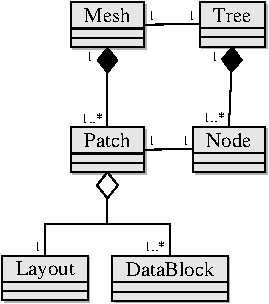
\includegraphics{uml/amr.1}}

%=======================================================================
\section{\code{Hierarchy} class}
%=======================================================================

A \code{Hierarchy} class represents a distributed structured AMR grid
hierarchy.  A \code{Hierarchy} can be considered to be an aggregate of
\code{Level}s, each of which in turn is an aggregate of individual
\code{Patch}es.  A patch is composed of a \code{Box}, which defines
the position and size in space, and some number of \code{Array}s, which
are used to store \code{Field} data (see \S\ref{ss:field}).



\subsection{Attributes}

\subsection{Operations}

%=======================================================================
\section{\code{Level} class}
%=======================================================================

A \code{Level} class represents a level in a distributed structured
AMR grid hierarchy (\code{Hierarchy}, where a level is defined as all
grid patches (\code{Grid}s) that have the same resolution.  A
\code{Level} is usually contained in a \code{Hierarchy}.

% The AMR hierarchy is represented using the trio of classes
% \code{Hierarchy}, \code{Level}, and \code{Grid}.
%   A \code{Grid} is a
% box in space, and is decomposed into \code{GridLocal} and
% \code{GridRemote} classes (see \S\ref{sss:class-grid}).  Each
% \code{GridLocal} object has some number of \code{Field} objects
% associated with them (see \S\ref{sss:class-field}), though the
% \code{GridLocal} objects themselves do not store field data
% themselves.  A \code{Level} class is also either a ``structured''
% \code{LevelStruct} or an ``unstructured'' \code{LevelUnstruct}.
% Structured levels are composed of a regular array of \code{Grid}s, and
% is typically used for unigrid calculations or the root level of an AMR
% calculation.  Unstructured levels are typically used for non-root
% levels of an AMR calulation.

\subsection{Attributes}

\subsection{Operations}

%=======================================================================
\section{\code{Patch} class}
%=======================================================================

A \code{Patch} class represents a grid patch in a distributed structured
AMR grid hierarchy (\code{Hierarchy}).  A \code{Patch} is defined by a
\code{Box}, and a set of \code{Array}s defined on the \code{Patch}.  Each
\code{Patch} is contained within a \code{Level}, and may be distributed
according to a \code{Parallel} object \S\ref{ss:parallel}.

\subsection{Attributes}

\subsection{Operations}

%=======================================================================
\section{\code{Box} class}
%=======================================================================

The \code{Box} class is for representing a box, and provides KeLP-like functionality.
Boxes are determined by two points, which may be of any parameterized type
(e.g.~\code{int} or \code{double}, etc.).


\subsection{Attributes}

\subsection{Operations}

%=======================================================================
\section{\code{Array} class}
%=======================================================================

The \code{Array} class encapsulates Fortran-style arrays with
convenient operations.  \code{Array}s may have optional support for
storing blocked or chunked arrays, include array padding, or store
interleaved arrays.  Arrays may be parallelized according to an
associated (static?) \code{Parallel} object (\S\ref{ss:parallel}).

% \centerline{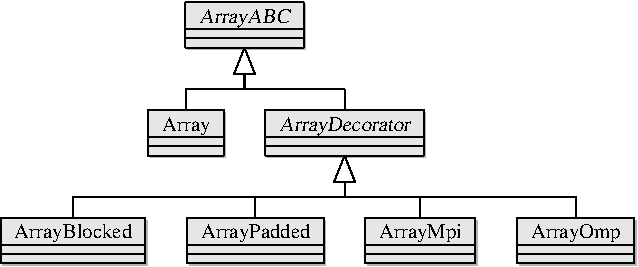
\includegraphics{uml/arrays.1}}

% \centerline{\includegraphics{uml/arrayabc.1}}

\centerline{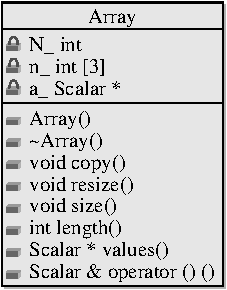
\includegraphics{uml/array.1}}

\subsubsection{Array shape}

\subsubsection{Array blocking}

\subsubsection{Array padding}

\subsubsection{Array interleaving}


\subsection{Attributes}

\begin{tabbing}
xx\=xx\=xxxxxxxxxxxxxxxxxxxxxxxxxxxxxxxxxxx\= \kill
\> \todo \>  \textit{Length of array} \\
\>       \> \code{N\_: int }      \\ \\
\> \todo \>  \textit {Shape of array, right-padded with 1's} \\
\>       \> \code{n\_: int [3] }  \\ \\
\> \todo \>  \textit {Array values stored in column-major ordering}\\
\>       \> \code{a\_: Scalar * }
\end{tabbing}

\subsection{Operations}

\begin{tabbing}
xx\=xx\=xxxxxxxxxxxxxxxxxxxxxxxxxxxxxxxxxxx\= \kill
\> \todo \> \textit{Create a new uninitialized Array object} \\
\>       \> \code{Array()} \\ \\
\> \todo \> \textit{Create a new initialized Array object} \\
\>       \> \code{Array(int n0, int n1=1, int n2=1, int n3=1)} \\ \\
\> \todo \> \textit{Deallocate the array} \\
\>       \> \code{\~{\ }Array()}  \\ \\
\> \todo \> \textit{Copy an array into this one, deallocating any existing data} \\
\>       \> \code{void copy (const Array \&)}  \\ \\
\> \todo \> \textit{Resize the array, deallocating any existing data} \\
\>       \> \code{void resize (int n0, int n1=1, int n2=1, int n3=1)}   \\ \\
\> \todo \> \textit{Return the size of the array} \\
\>       \> \code{void size (int *n0, int *n1=0, int *n2=0, int *n3=0) const}  \\ \\
\> \todo \> \textit{Return the total length of the array} \\
\>       \> \code{int length () const}  \\ \\
\> \todo \> \textit{Return a pointer to the array values} \\
\>       \> \code{Scalar * values () const}  \\ \\
\> \todo \> \textit{Return the given array element} \\
\>       \> \code{Scalar \& operator () (int i0, int i1=0, int i2=0, int i3=0)}
\end{tabbing}
%==================================================================
\end{document}
%==================================================================

